\chapter{Technische und fachliche Grundlagen} 
\label{ch:grundlagen}
Der dritte Teil dieser Diplomarbeit vermittelt die technischen Grundlagen für einige ausgewählte Bereiche und bereitet die Basis für das Verständnis der gewählten Konzepte in Teil vier. Die Untergliederung in Softwarearchitekturen, System Kommunikation, Datenbanksysteme und Konzepte stellt dabei nur eine grundlegende Einteilung dar und bilden einen Querschnitt durch wichtige Bereiche der Anwendungsarchitektur. Die Aufzählung stellt dabei keinen Anspruch auf Vollständigkeit und die Beschreibungen können nicht bis ins kleinste Detail vollzogen werden, da dies den Rahmen dieser Arbeit sprengen würde. Die Darstellung soll jedoch tiefgründig genug sein, um dem Leser ein fundiertes Verständnis der einzelnen Thematiken zu vermitteln.

\section{Softwarearchitekturen}
Die Definitionen, was Softwarearchitektur ist unterscheidet sich bei einzelnen Autoren. \citet*[S. 4]{Bass.2013} verwenden für mich eine sehr passende Definition des Begriffes:
	\begin{quote} 
	The software architecture of a system is the set of structures needed to reason about the system, which comprise software elements, relations among them, and properties of both.
	 \end{quote}
Vor allem die Zusammenhänge sind hier von Bedeutung, auch wenn das Design der Architektur nicht endgültig sein muss und sich im Laufe der Entwicklung noch Veränderungen und Anpassungen ergeben könne, so ist es doch von Anfang an wichtig eine Vorstellung über die geplanten Zusammenhänge im gesamten Team zu entwickeln.\\
Ich will daher hier drei grundlegende Architekturen darstellen, die sich in den Zusammenhängen unterscheiden. Jede diese Architekturen lässt sich in optimieren, anpassen und so besser nutzbar machen und oftmals gibt es auch unterschiedliche Kombinationen die zum gewünschten Erfolg führen.
	\subsection{Monolitisch}
	\subsection{Client/Server-Architekturmodell}
	Im Gegensatz zur monolitischen Architektur handelt es sich beim Client/Server Modell um ein verteiltes System.\\
	Das Client/Server-Architekturmodel ist ein Systemmodell, das aus einer Anzahl von zugehörigen Diensten und Servern besteht, sowie aus Clients, die diese Dienste nutzen und auf sie zugreifen. Das einfachste Modell ist dabei das zweischichtige Client/Server Modell, die zusammen ein komplettes System bilden mit unterschiedlichen Zuständigkeiten. \\
	Dabei lassen sich drei logische Hauptbestandteile unterschieden.
	
	\begin{figure}[h]
		\centering
		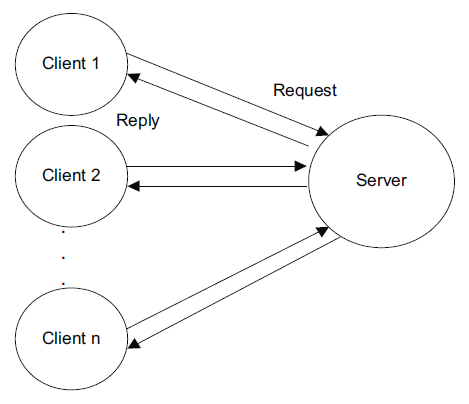
\includegraphics[width=0.7\linewidth]{images/Clients-und-Server}
		\caption{Client Server Model}
		\label{fig:client-server}
	\end{figure}
	
	\paragraph{Server}
	Der Server ist die zentrale Einheit der Architektur. Sie stellt Services und Daten anderen Einheiten zur Verfügung. Der Server muss nicht zwingend wissen, welche und wie viele Einheiten die von ihm zur Verfügung gestellten Dienste und Daten nutzen.
	
	\paragraph{Client}
	Clients können in beliebig großer Anzahl existieren. Sie nehmen die Daten oder Services, die vom Server bereitgestellt werden in Anspruch. Um mit den Diensten interagieren zu können, muss ein Client von der Existenz und dessen Adresse wissen. Der Client sendet eine Anfrage an den Server und bekommt ein Resultat zurück geliefert. \citet*[S. 302]{Sommerville.2007} unterscheidet folgende zwei Client-Modelle:
	\subsubsection{Thin-Client-Modell}
	Bei diesem Modell werden die gesamten Anwendungsprozesse und Datenhaltung auf dem Server erledigt. Der Client ist nur für die Darstellung verantwortlich. Daraus ergibt sich der Vorteil, dass sehr wenig Ressourcen für den Client benötigt werden und dieser sich auch auf kleinen Systemen (z.B. Terminals) implementieren lässt. Der Nachteil dieses Modelles liegt jedoch darin, dass so sämtliche Arbeit Serverseitig geleistet werden muss. Gerade bei Anwendungen mit großer Client Anzahl oder rechenintensiven Operationen kann so der Server schnell zur kritischen Komponente werden und das System vor Skalierungsprobleme stellen. Zusätzlich führt der Thin-Client zu einer erhöhten Netzwerkbelastung, da alle Daten vom Server zum Client transportiert werden müssen.
	
	\subsubsection{Fat-Client-Modell}
	Dieses Modell verlagert die Anwendungslogik vollständig oder in großen Teilen vom Server direkt in den Client. Dadurch kann der Server deutlich entlastet werden und die Rechenleistung des Client Rechners zusätzlich genutzt werden. Dies kann sich in speziellen Situationen allerdings auch als Nachteile erweisen, wenn die Client Computer die notwendige Rechenleistung nicht selbstständig bereitstellen könne. Der Server fungiert dabei nur noch als Daten Service und die Netzwerklast wird reduziert. Die Verlagerung der Anwendungslogik auf den Client bringt aber auch Nachteile mit sich. Müssen hier Änderungen vorgenommen werden, so müssen alle Clients auf die neue Version aktualisiert werden, was zu einem komplexen Systemmanagement führen kann. Der Aufwand dafür steigt mit zunehmender Zahl der Clients.
	
	\paragraph{Netzwerk (optional)}
	In der Literatur wird das Netzwerk häufig noch ein dritter Bestandteil aufgeführt, der jedoch nicht zwingend notwendig ist da prinzipiell Server und Client auf einem Computer ausgeführt werden können und so kein Netzwerk zur Kommunikation benötigen. Da dieses Modell aber in der Praxis nahezu ausschließlich als verteiltes System angewendet wird, ist in diesen Fällen das Netzwerk grundlegende Kommunikationsgrundlage.
	\\
	
	Generell hat das zweischichtige Client/Server Modell das Problem, dass die drei logischen Schichten auf zwei unterschiedlichen Computersystemen abgebildet werden müssen. \\
	
	\begin{figure}[h]
		\centering
		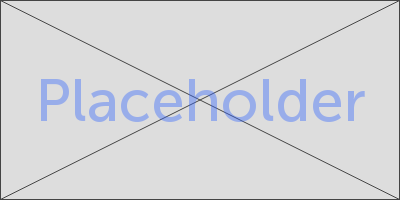
\includegraphics[width=0.7\linewidth]{images/placeholder}
		\caption{Logische drei Schichten}
		\label{fig:log3schichten}
	\end{figure}
	
	Als Alternativansatz hat sich dafür die dreischichtige Architektur Entwickelt. Sie stellt für jede logische Schicht ein separates Computersystem zur Verfügung. Die Vorteile liegen dabei in der besseren Skalierbarkeit, da jedes System individuell skaliert werden kann, geringere Netzwerklast im Vergleich zum Thin-Client-Modell und Anwendungsprozesse sind zentralisiert und lassen sich dort leichter anpassen und aktualisieren.
	

	\begin{figure}[h]
		\centering
		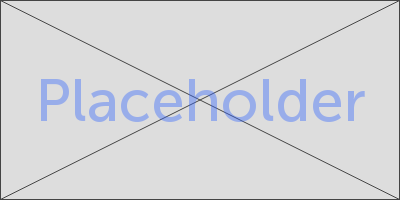
\includegraphics[width=0.7\linewidth]{images/placeholder}
		\caption{Drei schichtige Architektur}
		\label{fig:3-tier-architecture}
	\end{figure}


	Sommerville gibt in seinem Buch Software Engineering Beispiele, wann die Anwendung der jeweiligen Architektur sinnvoll ist.
	
	
	\begin{tabular}{|p{3.5cm}|p{12.5cm}|}
		\hline 
		Architektur & Anwendung \\ 
		\hline 
		Zweischichtige C/S-Architektur mit Thin-Clients & Anwendungen mit Legacy-Systemen, bei denen die Trennung von Anwendungsprozessen und Datenmanagement nicht praktikabel ist Rechenintensive Anwendungen wie zum Beispiel Compiler mit geringem oder keinem Datenmanagement -Datenintensive Anwendungen (Browser oder Abfragesysteme) mit wenig oder keinen Anwendungsprozessen \\
		\hline 
		Zweischichtige C/S-Architektur mit Fat-Clients & Anwendungen, bei denen die Prozesse durch Standardanwendungen (z.b. Microsoft Excel) auf dem Client verarbeitet werden Anwendungen mit rechenintensiver Datenverarbeitung (z.B. Datenvisualisierung) Anwendungen mit relativ stabiler Endbenutzerfunktionalität, die in einer Umgebung mit gut strukturiertem Systemmanagement angeordnet sind \\ 
		\hline 
		Drei- oder mehrschichtige C/S-Architektur & Anwendungen großen Umfangs mit Hunderten oder Tausenden von Clients Anwendungen, bei denen sowohl die Daten als auch die Anwendung selbst ständigen Veränderungen unterliegen Anwendungen, bei denen Daten aus vielfältigen Quellen verarbeitet werden \\ 
		\hline 
	\end{tabular} 
	
	
	
	\subsection{Dienstorientiert}

\section{System Kommunikation}
	\subsection{Represental State Transfer (REST)}
	\subsection{Remote Procedure Call (RPC)}
	\subsection{Enterprise Service Bus (ESB)}
	\subsection{Message Bus}

\section{Datenbanksysteme}
	\subsection{Relationale Datenbanken}
	\subsection{NoSQL Datenbanken}
	\subsection{Gegenüberstellung}
	
\section{Konzepte}
	\subsection{Singel Responisibility}
	\subsection{Domain Driven Design}
	\subsection{Data Consistency Primer}
	\subsection{Competiting Consumer Pattern}
	\subsection{Materialized View Pattern}
	\subsection{Queue-Based Lode Leveling Pattern}
	\subsection{Api Gateway Pattern}
